\section{Methodology of LSTM}
LSTM is a special kind of Recurrent Neural Network(RNN) \cite{sak2014long}. It is able to learn from sequential data quickly and capture both short-term and long-term dependencies in sequential data. Because LSTM involves the memory cell which is composed of input gate, forget gate and output gate.

\begin{figure}[ht]
    \centering
    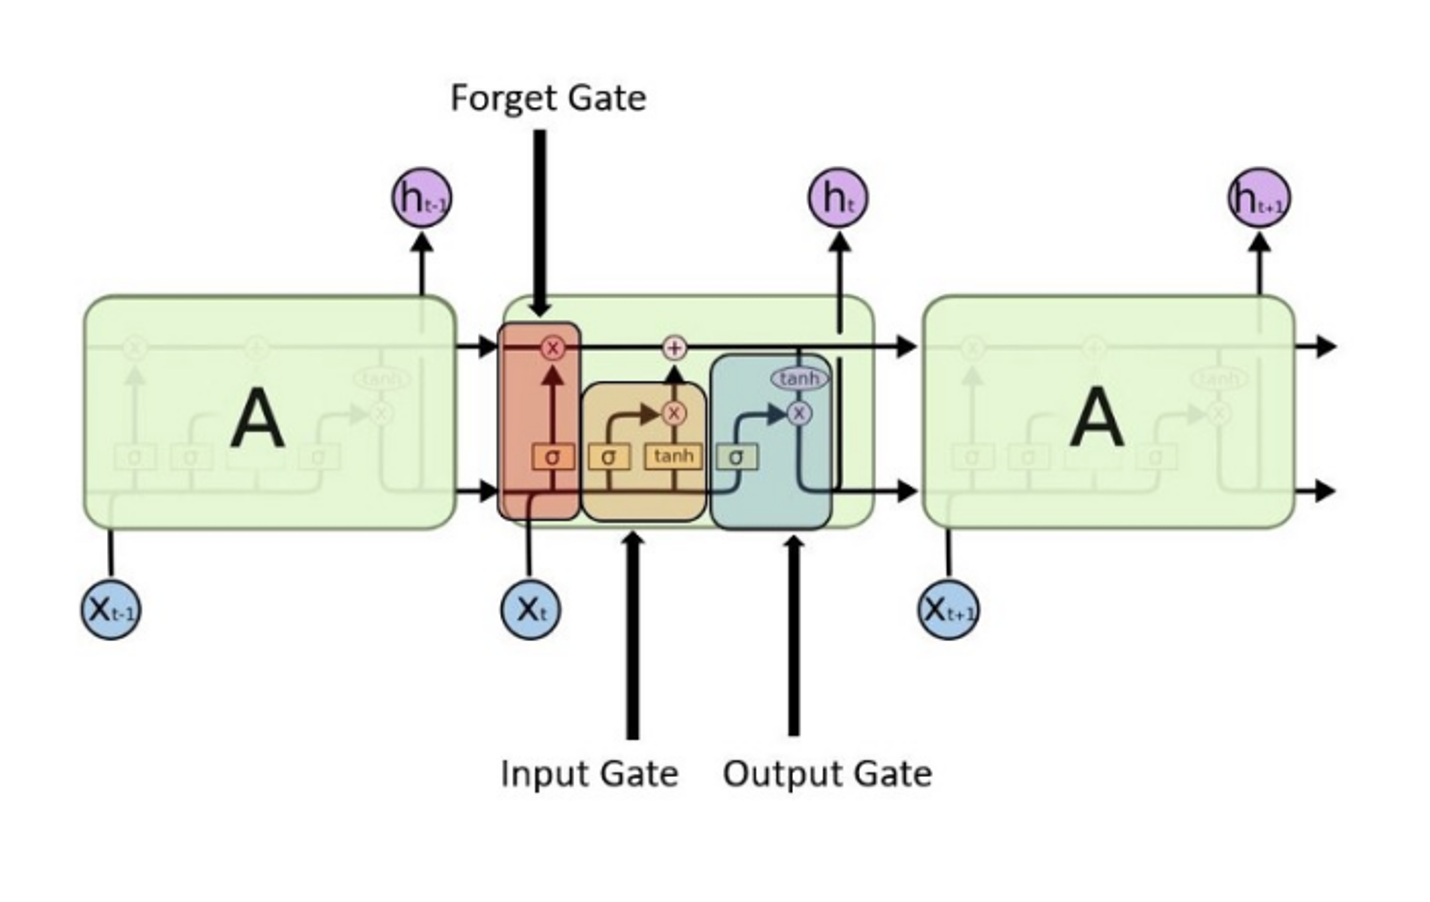
\includegraphics[width=0.5\textwidth]{pics/lstm_architecture.png}
    \caption{The architecture of LSTM}
\end{figure}

A cell state through gates allow LSTM to selectively retain or discard information and make it performing well in natural language text. LSTM can automatically learn features from raw sequences so that we don't need to construct features like n-gram and TF-IDF. Furthermore, compared to standard Recurrent Neural Networks, LSTMs are specifically designed to address the vanishing gradient problem, which allows them to remember information across longer text spans, a crucial advantage for sentiment analysis tasks.

\subsection{Model Architecture of LSTM}
We built the LSTM model with the following steps: processed raw IMDB data into padded integer sequences, added embedding and LSTM layer to extract features, then regularized with dropout, and finally get sentiment classification through a sigmoid activated dense layer.

\begin{figure}[ht]
    \centering
    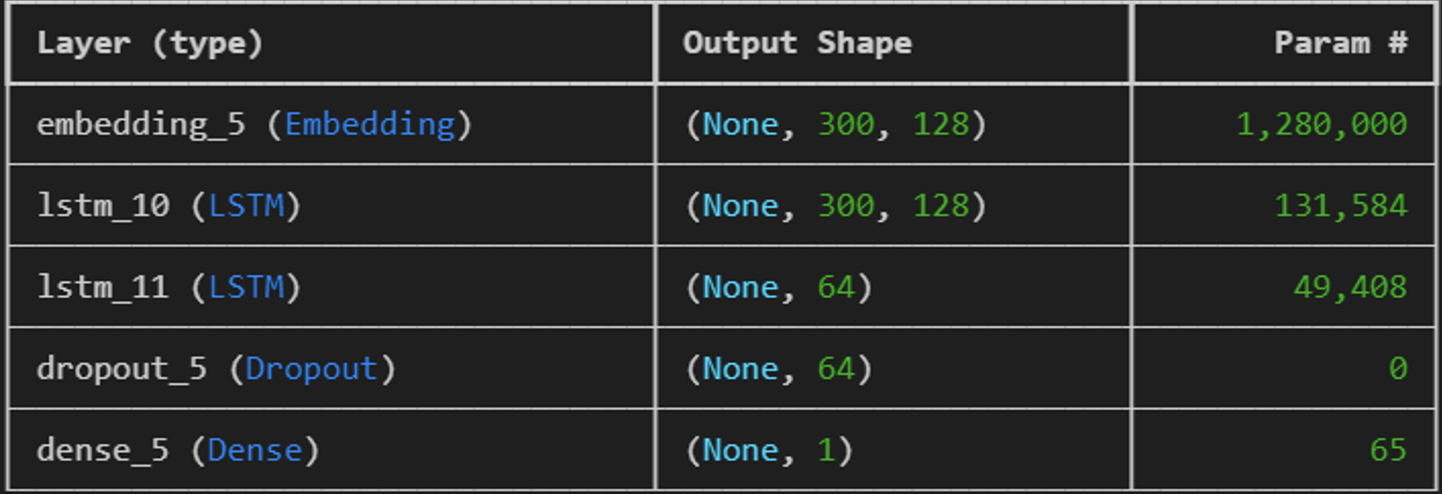
\includegraphics[width=0.6\textwidth]{pics/lstm_model.png}
    \caption{The model review of LSTM}
\end{figure}

The pipeline began with raw IMDB reviews. We proprocessed the data by mapping each word into an integer index and then padding all sequences to a length of 300 tokens. This allowed the data to be trained efficiently in batches. Next we built an Embedding layer, which serves as the input layer. It transforms the integer-encoded vocabulary (limited to the 10,000 most frequent words) into dense, 128-dimensional vectors. This layer is crucial as it learns a meaningful, continuous representation for each word that captures semantic relationships within the vector space.

Next, we stack two LSTM layers to model temporal dependencies in the text. The first LSTM has 128 hidden units and it outputs the entire sequence of hidden states. This seconde LSTM layer has 64 hidden units and outputs only a hidden state from the finnal time step. This single vector acts as a powerful summary of the entire input sequence, encoding the sentiment of the review.

To reduce the risk of overfitting, we inserted a dropout layer with a rate of 0.4 between the LSTM stack and the final dense output layer. The last layer used a single neuron with a sigmoid activation function to predict the probability of the review being positive. The training was performed using the Adam optimizer and binary cross-entropy loss, with model performance evaluated through both accuracy and AUC metrics.

\subsection{Results and Experiments of LSTM}
After training 50 epochs of our LSTM model, we evaluated it on an unseen test set. Our model got 85.5\% accuracy in the test set and a Test Area Under the Curve (AUC) of 88\%. This indicated that our LSTM model has successfully learned sentiment-relevant features from the data.

The classification report showed almost similar precision, recall, and F1-scores for both positive and negative classes. They all approached around 0.855 which indicates that the model treated both positive and negative reviews with equal effectiveness and no bias.

\begin{figure}[ht]
    \centering
    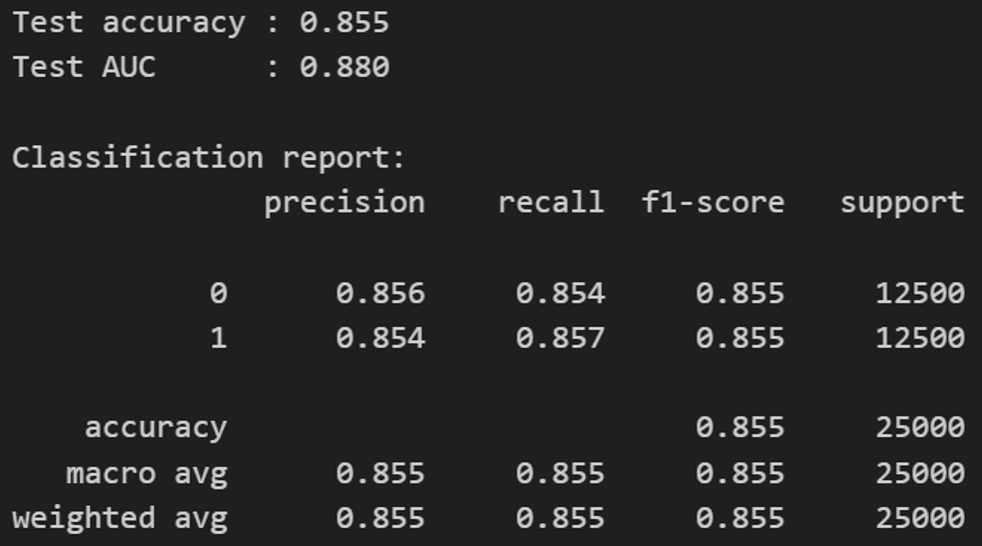
\includegraphics[width=0.5\textwidth]{pics/lstm_report.png}
    \caption{The classification report of LSTM}
\end{figure}

In the confusion matrix, the diagonal values (TN, TP) are much higher than off-diagonal (FP, FN) which shows a high correct rate prediction along the main diagonal versus incorrect predictions. The number of False Positives and False Negatives is very similar, 1827 and 1791 respectively. This balance also supported that the model's errors were not biased towards any one class.

\begin{figure}[ht]
    \centering
    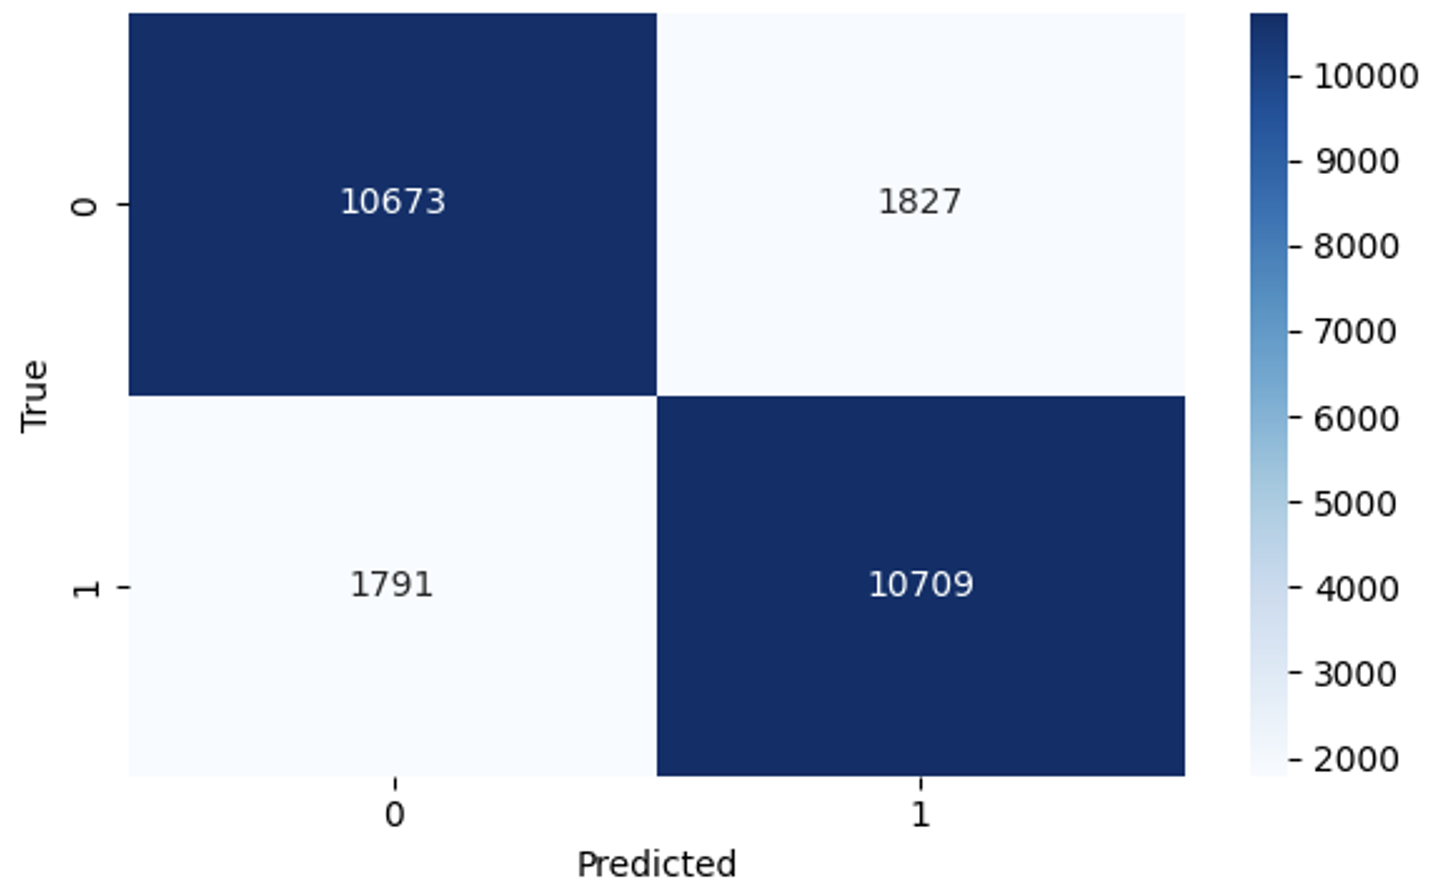
\includegraphics[width=0.5\textwidth]{pics/lstm_metrix.png}
    \caption{The confusion matrix of LSTM}
\end{figure}

In the "Accuracy on epochs" plot, we can clearly see the learning curve of our LSTM model.  From the training and validation accuracy curves, it is observed that the validation accuracy stabilizes after the 15th epoch, while the training accuracy continues to rise. This phenomenon suggests a risk of overfitting but can be controlled by regularization and monitoring.

\begin{figure}[ht]
    \centering
    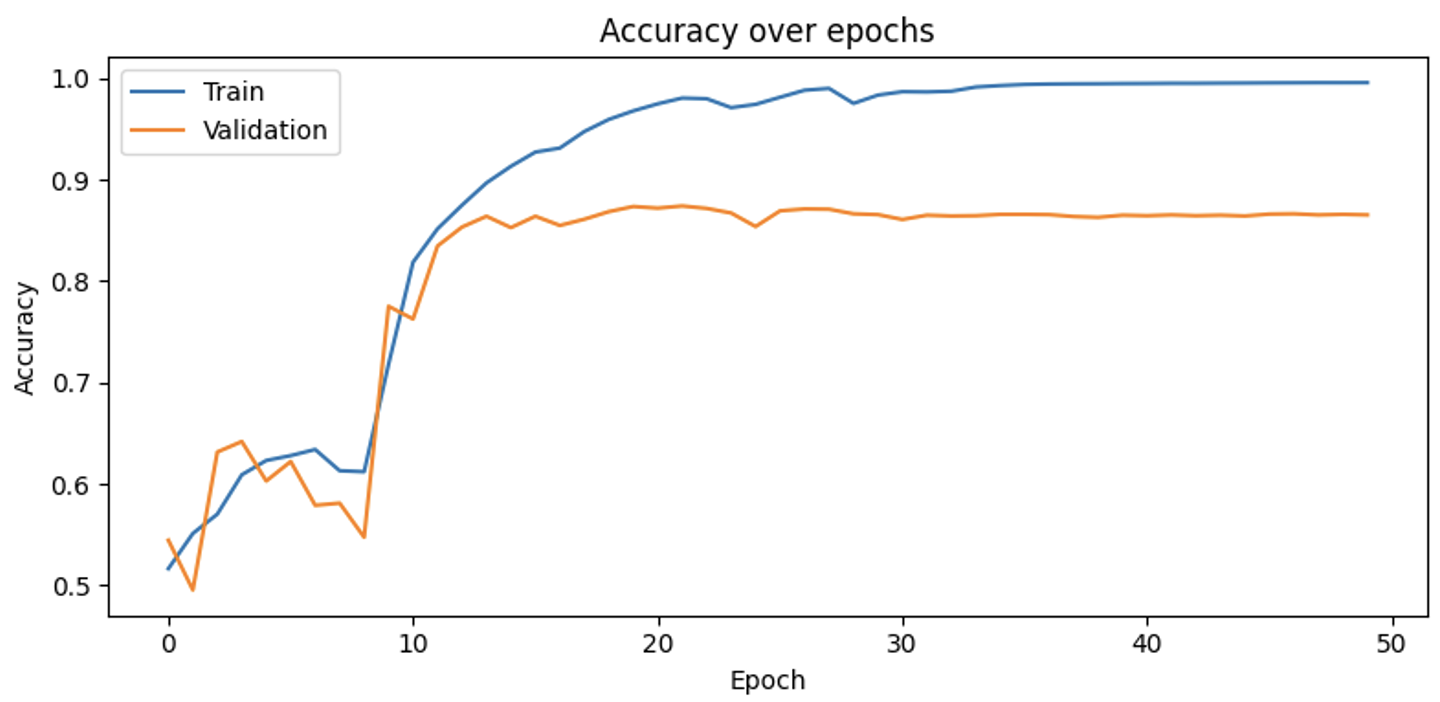
\includegraphics[width=0.5\textwidth]{pics/lstm_accuracy_s.png}
    \caption{Accuracy on epochs of LSTM}
\end{figure}

In summary, LSTM networks offer a powerful and balanced solution for sentiment analysis on the IMDB dataset that outperforms traditional methods and achieves robust and unbiased results. In the future, we can try to make some improvements including the integration of pre-trained word vectors, attention mechanisms, or more sophisticated regularisation techniques, as well as a more formal assessment of the model's statistical significance and generalisation capabilities.





